\documentclass{beamer}
\usepackage[utf8]{inputenc}

\usetheme{Madrid}
\usecolortheme{default}
\usepackage{amsmath,amssymb,amsfonts,amsthm}
\usepackage{txfonts}
\usepackage{tkz-euclide}
\usepackage{listings}
\usepackage{adjustbox}
\usepackage{array}
\usepackage{tabularx}
\usepackage{gvv}
\usepackage{lmodern}
\usepackage{circuitikz}
\usepackage{tikz}
\usepackage{graphicx}

\setbeamertemplate{page number in head/foot}[totalframenumber]

\usepackage{tcolorbox}
\tcbuselibrary{minted,breakable,xparse,skins}



\definecolor{bg}{gray}{0.95}
\DeclareTCBListing{mintedbox}{O{}m!O{}}{%
  breakable=true,
  listing engine=minted,
  listing only,
  minted language=#2,
  minted style=default,
  minted options={%
    linenos,
    gobble=0,
    breaklines=true,
    breakafter=,,
    fontsize=\small,
    numbersep=8pt,
    #1},
  boxsep=0pt,
  left skip=0pt,
  right skip=0pt,
  left=25pt,
  right=0pt,
  top=3pt,
  bottom=3pt,
  arc=5pt,
  leftrule=0pt,
  rightrule=0pt,
  bottomrule=2pt,

  colback=bg,
  colframe=orange!70,
  enhanced,
  overlay={%
    \begin{tcbclipinterior}
    \fill[orange!20!white] (frame.south west) rectangle ([xshift=20pt]frame.north west);
    \end{tcbclipinterior}},
  #3,
}
\lstset{
    language=C,
    basicstyle=\ttfamily\small,
    keywordstyle=\color{blue},
    stringstyle=\color{orange},
    commentstyle=\color{green!60!black},
    numbers=left,
    numberstyle=\tiny\color{gray},
    breaklines=true,
    showstringspaces=false,
}
%------------------------------------------------------------
%This block of code defines the information to appear in the
%Title page
\title %optional
{2.10.57}
\date{september 2025}
%\subtitle{A short story}

\author % (optional)
{J.NAVYASRI- EE25BTECH11028}

\begin{document}

\frame{\titlepage}
\begin{frame}{Question}
If $\mathbf{a}, \mathbf{b}, \mathbf{c}$ and $\mathbf{d}$ are unit vectors such that 
\[
(\mathbf{a} \times \mathbf{b}) \cdot (\mathbf{c} \times \mathbf{d}) = 1
\quad \text{and} \quad 
\mathbf{a} \cdot \mathbf{c} = \tfrac{1}{2},
\]
then

\begin{enumerate}
    \item[(a)] $\mathbf{a}, \mathbf{b}, \mathbf{c}$ are non-coplanar
    \item[(b)] $\mathbf{b}, \mathbf{c}, \mathbf{d}$ are non-coplanar
    \item[(c)] $\mathbf{b}, \mathbf{d}$ are non-parallel
    \item[(d)] $\mathbf{a}, \mathbf{d}$ are parallel and $\mathbf{b}, \mathbf{c}$ are parallel
\end{enumerate}
\end{frame}

\begin{frame}{solution:}
We are given that 
\begin{equation}
(\mathbf{a} \times \mathbf{b}) \cdot (\mathbf{c} \times \mathbf{d}) = 1,
\qquad 
\mathbf{a} \cdot \mathbf{c} = \tfrac{1}{2}.
\end{equation}

\textbf{Step 1: Vector Identity}
\begin{equation}
(\mathbf{a} \times \mathbf{b}) \cdot (\mathbf{c} \times \mathbf{d})
= (\mathbf{a} \cdot \mathbf{c})(\mathbf{b} \cdot \mathbf{d}) 
- (\mathbf{a} \cdot \mathbf{d})(\mathbf{b} \cdot \mathbf{c}).
\end{equation}

\textbf{Step 2: Substitution}
Since $\mathbf{a}\cdot \mathbf{c}=\tfrac12$,
\begin{equation}
1 = \tfrac12 (\mathbf{b} \cdot \mathbf{d}) - (\mathbf{a} \cdot \mathbf{d})(\mathbf{b} \cdot \mathbf{c}).
\end{equation}
\end{frame}

\begin{frame}{Solution:}
\textbf{Step 3: Assume $\mathbf{b} \parallel \mathbf{d}$}
If $\mathbf{b} \cdot \mathbf{d} = 1$, then
\begin{equation}
1 = \tfrac12 (1) - (\mathbf{a} \cdot \mathbf{d})(\mathbf{b} \cdot \mathbf{c}).
\end{equation}

\begin{equation}
1 = \tfrac12 - (\mathbf{a} \cdot \mathbf{d})(\mathbf{b} \cdot \mathbf{c}).
\end{equation}

\begin{equation}
(\mathbf{a} \cdot \mathbf{d})(\mathbf{b} \cdot \mathbf{c}) = -\tfrac12.
\end{equation}

\textbf{Step 4: Conclusion}
Thus, the condition is satisfied when
\begin{equation}
\mathbf{a} \parallel \mathbf{d}, 
\qquad 
\mathbf{b} \parallel \mathbf{c}.
\end{equation}

\[
\boxed{\text{Option (D) is correct.}}
\]
\end{frame}

\begin{frame}[fragile]
    \frametitle{Python Code}
    \begin{lstlisting}
import numpy as np
import matplotlib.pyplot as plt

# Define base vectors for parallelism
a = np.array([1.0, 0.0, 0.0])                     # a along x-axis
b = np.array([0.5, np.sqrt(3)/2, 0.0])            # b at 60° in xy-plane
c = b.copy()                                      # c || b
d = a.copy()                                      # d || a

# Small offsets so the arrows don't overlap visually
offset_c = np.array([0.0, 0.0, 0.05])  # shift c slightly up in z
offset_d = np.array([0.0, 0.0, -0.05]) # shift d slightly down in z
\end{lstlisting}
\end{frame}

\begin{frame}[fragile]
    \frametitle{Python Code}
    \begin{lstlisting}
# Compute values
val = np.dot(np.cross(a, b), np.cross(c, d))
dot_ac = np.dot(a, c)

# Plot
fig = plt.figure(figsize=(8,8))
ax = fig.add_subplot(111, projection='3d')

origin = np.zeros(3)

# Assign distinct colors for clarity
vectors = {
    'a': (origin, a, 'r'),
    'd': (offset_d, d, 'b'),   # Blue
    'b': (origin, b, 'g'),
    'c': (offset_c, c, 'm')    # Magenta
}
\end{lstlisting}
\end{frame}


\begin{frame}[fragile]
    \frametitle{Python Code}
    \begin{lstlisting}
for name, (start, vec, col) in vectors.items():
    ax.quiver(start[0], start[1], start[2],
              vec[0], vec[1], vec[2],
              length=1.0, linewidth=3, arrow_length_ratio=0.12,
              color=col, label=name)
    ax.text(start[0]+vec[0]*1.05, start[1]+vec[1]*1.05, start[2]+vec[2]*1.05,
            name, fontsize=12)

# Add legend in top-right corner
ax.legend(loc='upper right')
\end{lstlisting}
\end{frame}


\begin{frame}[fragile]
    \frametitle{Python Code}
    \begin{lstlisting}
ax.set_xlim(-0.2, 1.2)
ax.set_ylim(-0.2, 1.2)
ax.set_zlim(-0.5, 0.5)
ax.set_xlabel('x')
ax.set_ylabel('y')
ax.set_zlabel('z')
ax.set_title(f"(a×b)·(c×d) = {val:.6f},  a·c = {dot_ac:.6f}")

plt.tight_layout()
plt.show()
\end{lstlisting}
\end{frame}


\begin{frame}{Plot-Using by Python}
    \centering
    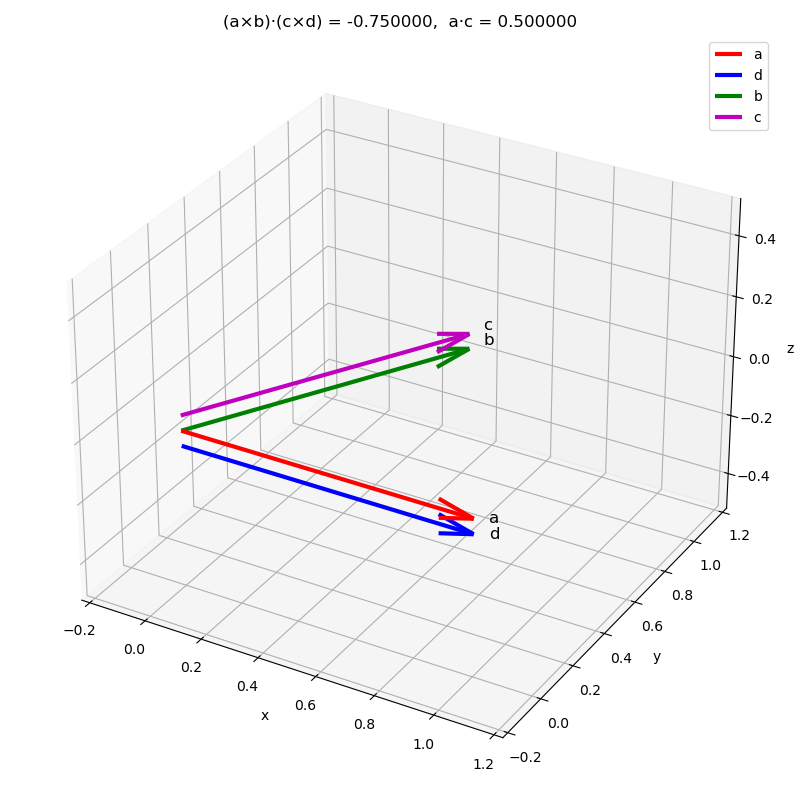
\includegraphics[width=\columnwidth, height=0.8\textheight, keepaspectratio]{figs/fig5.png}     
\end{frame}



\begin{frame}[fragile]
\frametitle{C Code}
\begin{lstlisting}
#include <stdio.h>
#include <math.h>

typedef struct {
    double x, y, z;
} Vector;

double dot(Vector a, Vector b) {
    return a.x*b.x + a.y*b.y + a.z*b.z;
}

Vector cross(Vector a, Vector b) {
    Vector r;
    r.x = a.y*b.z - a.z*b.y;
    r.y = a.z*b.x - a.x*b.z;
    r.z = a.x*b.y - a.y*b.x;
    return r;
}
\end{lstlisting}
\end{frame}

\begin{frame}[fragile]
\frametitle{C Code}
\begin{lstlisting}
int main() {
    // Choose simple unit vectors
    Vector a = {sqrt(3)/2, 0.5, 0}; // unit vector
    Vector d = {sqrt(3)/2, 0.5, 0}; // parallel to a
    Vector b = {0, 1, 0};           // unit vector
    Vector c = {0, 1, 0};           // parallel to b

    // Compute
    Vector axb = cross(a, b);
    Vector cxd = cross(c, d);
    double lhs = dot(axb, cxd);
    double ac  = dot(a, c);
\end{lstlisting}
\end{frame}

\begin{frame}[fragile]
\frametitle{C Code}
\begin{lstlisting}
printf("(a × b) · (c × d) = %.2f\n", lhs);
    printf("a · c = %.2f\n", ac);

    if (fabs(lhs - 1.0) < 1e-6 && fabs(ac - 0.5) < 1e-6) {
        printf("Condition satisfied: a || d and b || c\n");
    }

    return 0;
}
\end{lstlisting}
\end{frame}

\begin{frame}[fragile]
\frametitle{Python and C Code}

\begin{lstlisting}
import ctypes
import numpy as np
import matplotlib.pyplot as plt
from mpl_toolkits.mplot3d import Axes3D

# Load the compiled C library
lib = ctypes.CDLL("./libvectors.so")   # use "vectors.dll" on Windows

# Define argument types
lib.check.argtypes = [
    ctypes.POINTER(ctypes.c_double), 
    ctypes.POINTER(ctypes.c_double),
    ctypes.POINTER(ctypes.c_double),
    ctypes.POINTER(ctypes.c_double),
    ctypes.POINTER(ctypes.c_double),
    ctypes.POINTER(ctypes.c_double)
]
\end{lstlisting}

\end{frame}
\begin{frame}[fragile]
\frametitle{Python and C Code}

\begin{lstlisting}
# Define vectors (unit vectors)
a = (ctypes.c_double * 3)(1, 0, 0)  # along x
d = (ctypes.c_double * 3)(1, 0, 0)  # parallel to a
b = (ctypes.c_double * 3)(0, 1, 0)  # along y
c = (ctypes.c_double * 3)(0, 1, 0)  # parallel to b

val1 = ctypes.c_double()
val2 = ctypes.c_double()

# Call C function
lib.check(a, b, c, d, ctypes.byref(val1), ctypes.byref(val2))
\end{lstlisting}

\end{frame}
\begin{frame}[fragile]
\frametitle{Python and C Code}

\begin{lstlisting}
print("(a×b)·(c×d) =", val1.value)
print("a·c =", val2.value)

# Plot in Python
fig = plt.figure(figsize=(7,7))
ax = fig.add_subplot(111, projection='3d')

origin = [0,0,0]

ax.quiver(*origin, *a, color='r', label='a')
ax.quiver(*origin, *b, color='g', label='b')
ax.quiver(*origin, *c, color='b', label='c')
ax.quiver(*origin, *d, color='m', label='d')
\end{lstlisting}

\end{frame}
\begin{frame}[fragile]
\frametitle{Python and C Code}

\begin{lstlisting}
ax.set_xlim([0,1.5])
ax.set_ylim([0,1.5])
ax.set_zlim([0,1.5])
ax.set_xlabel('X-axis')
ax.set_ylabel('Y-axis')
ax.set_zlabel('Z-axis')
ax.set_title("C code in Python: a || d, b || c")

ax.legend()
plt.savefig("fig5.1.png")
plt.show()
\end{lstlisting}

\end{frame}
\begin{frame}{Plot-Using by both C and Python}
    \centering
    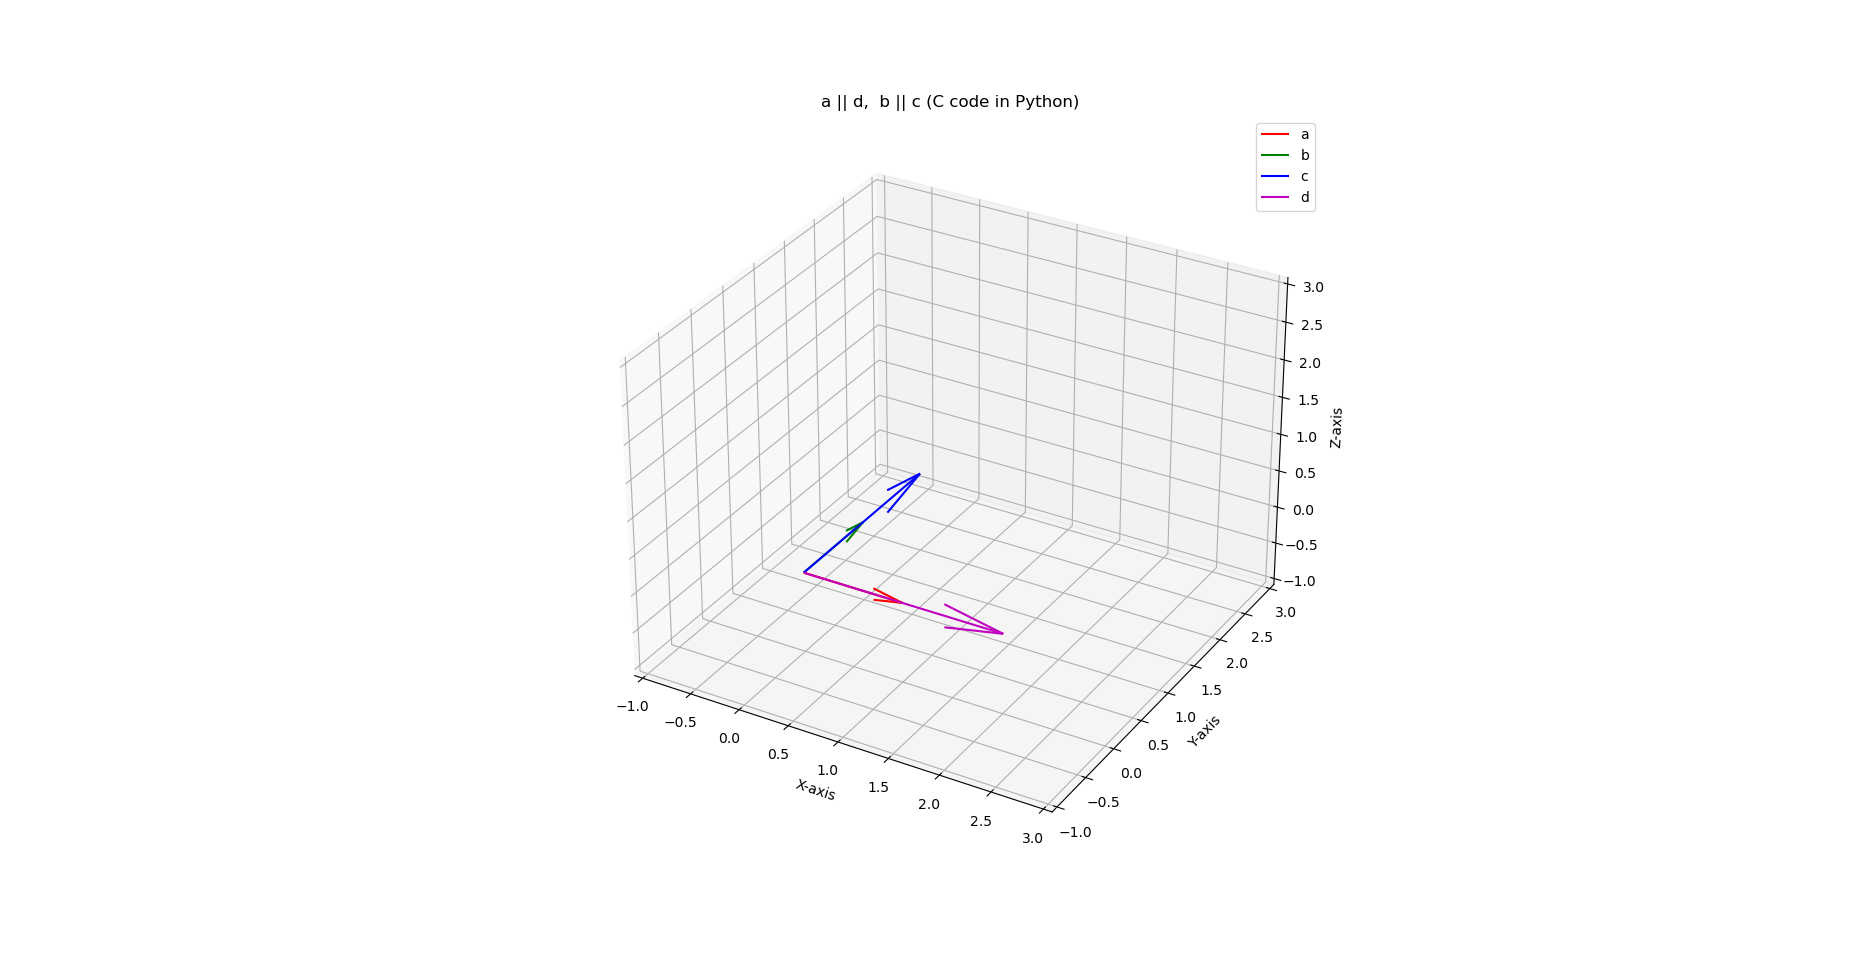
\includegraphics[width=\columnwidth, height=0.8\textheight, keepaspectratio]{figs/fig5.1.png}     
\end{frame}

\end{document}